\subsection{Transcriptional Changes of Human \textit{IFITs}} \label{Transcriptional Changes of Human IFITs}
To unravel the impact of cellular stimulation with activators of the innate immune response and human RSV, on the expression of human \textit{IFIT} genes, quantitative real-time reverse transcription PCR (qPCR) analysis was executed in accordance with the methodology outlined in Section \ref{Quantitative Real Time/Reverse Transcription PCR}. Briefly, cells were cultivated in 12-well plates and subsequently subjected to the respective stimulants. At the endpoint of the experiments, the RNA was extracted, followed by cDNA synthesis and the transcript quantification by qPCR. All transcript levels were standardized to human \textit{GAPDH} expression, employing  the 
\(\Delta\)\(\Delta\)Ct method. Subsequently, all values were normalized against mock-treated samples, enabling data aggregation and inter-experimental induction value comparison. The statistical analysis was conducted as outlined in Section \ref{Statistical Analysis}. Notably, the choice of the appropriate statistical test hinged on the normality of data distribution and equality of variance, aspects which will be underscored in the ensuing text.



\subsubsection{Human \textit{IFITs} Responses of to Known Activators of Innate Immune Response} \label{Human IFIT Responses to Known Activators of Innate Immune Response}
In order to establish the expression competency of human \textit{IFITs} of the A549 cell line, along with elucidating how different innate immune pathways contribute to the overall expression profile, I treated the cells with differing activators of the innate immune response. As described in Section \ref{Routes of IFIT Expression Activation}, and depicted in Figure \ref{Pathways Inducing ISG mRNA Production.},  interferon-stimulated genes (ISGs) can have their induction activated either via the interferon receptor signalling, intracellular foreign nucleic acid detection or via extracellular PAMP sensing. The latter, in the context of RSV, includes stimulation of TLR4 with either LPS or RSV particles. After surveying the literature I ended up using 1,000 international units (IU) per mL of human interferon alpha (\cite{Terenzi2006DistinctISG56}; \cite{Santhakumar2018ChickenViruses}). For interferon-gamma stimulation, which stimulates predominantly immune cells \textit{in vivo} concentrations of 500, 1,000 and 2,000 IU/mL were used. LPS was administered in concentrations of 5 ng/mL and 5 \(\mu\)g/mL for the duration of 6 hours. (\cite{Mears2019Ifit1Cells}; \cite{Zhang2019GrouperResponse}). To stimulate intracellular foreign nucleic acid recognition 2 \(\mu\)g of poly I:C were transfected into A549 cells and incubated for 24 hours (\cite{Mears2019Ifit1Cells}; \cite{Palchetti2015TransfectedCells}).

\begin{figure}
    \centering
    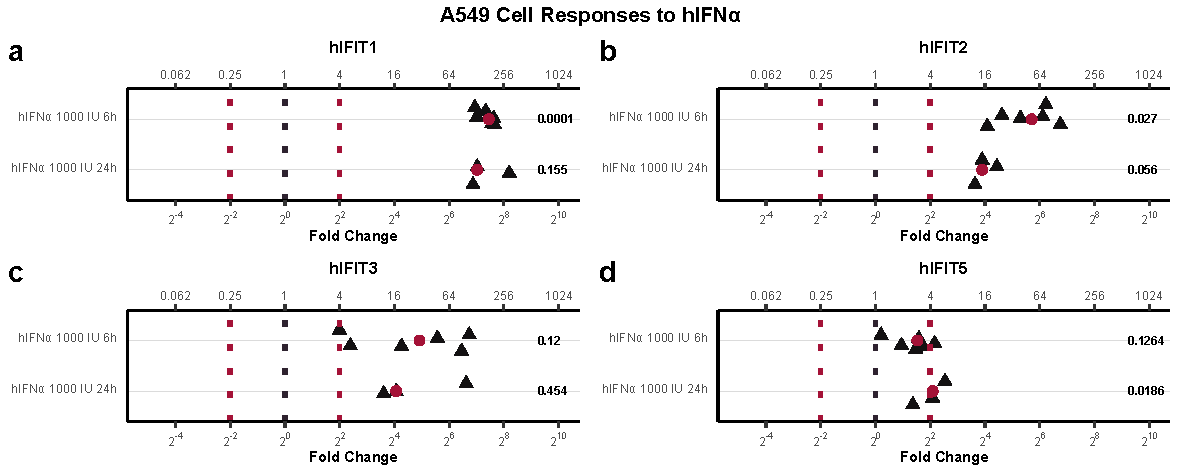
\includegraphics[width=1\linewidth]{06. Chapter 1/Figs/01. Induction/01. a549_treat_ifna.pdf}
    \caption[qPCR Analysis of A549 \textit{hIFIT} Response to hIFN\(\alpha\).]{\textbf{qPCR Analysis of A549 \textit{hIFIT} to hIFN\(\alpha\).} The relative abundance of (a) \textit{hIFIT1}, (b) \textit{hIFIT2}, (c) \textit{hIFIT3}, and (d) \textit{hIFIT5} genes, extracted from the A549 cell line, with response to human interferon alpha (IFN\(\alpha\)) at a concentration of 1000 IU per mL for a treatment duration of 6 or 24 hours. The shown values are relative to standardised mock values. The red circles signify median values. The black dotted line indicates mock expression, while the red dotted lines indicate biologically significant levels of induction. Numeric values signify the p-values compared to mock.}
    \label{A549 Response to hIFNa}
\end{figure}

The A549 cell line, derived from   lung carcinomatous tissue from a 58-year-old Caucasian male in 1972 is a well-established model of alveolar epithelial cells, routinely used for cancer to viral research alike (\cite{Lieber1976ACells}). We observe that after the stimulation of the A549 cell line with 1,000 IU/mL of hIFN\(\alpha\) for either 6 or 24 hours human \textit{IFIT1}, \textit{IFIT2}, and \textit{IFIT3} were induced drastically, especially \textit{IFIT1}, which was induced around 200-fold (Figure \ref{A549 Response to hIFNa}). The relative induction levels were identical between \textit{IFIT2} and \textit{IFIT3}. For all of these 3 genes, we can observe a decreased expression with longer incubation of IFN\(\alpha\), i.e. approximately half of the induction levels caused by 6-hour long incubation. Human \textit{IFIT5} shows minimal induction compared to the other \textit{IFITs} (3 and 4-fold for 6 and 24-hour long incubation respectively), which hovers around the mark of what is considered biologically significant induction, especially for ISGs, which are supposed not to be highly basally expressed. We can also observe a reverse trend of the time dependency of hIFN\(\alpha\)-induced expression. This suggests differential induction sensitivities between \textit{hIFIT1} (highly induced), \textit{hIFIT2} and \textit{hIFIT3} (medium induced) and \textit{hIFIT5} (low induced). All \textit{hIFIT} values had normal distributions and unequal variance other than \textit{hIFIT5}, which had normal distribution and normal variance.

\begin{figure}
    \centering
    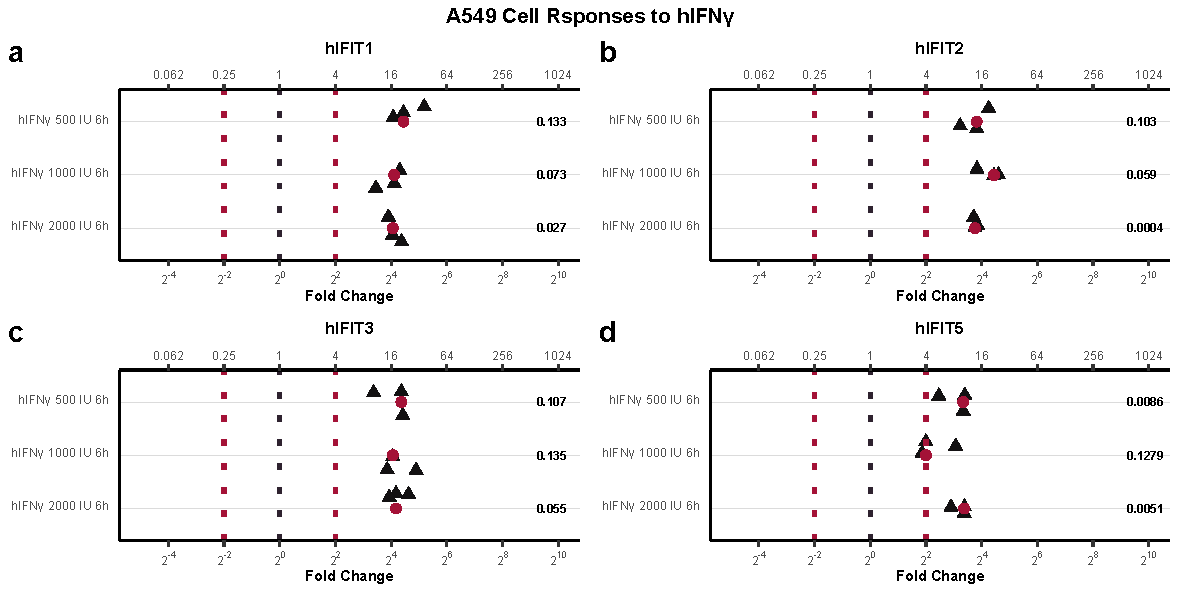
\includegraphics[width=1\linewidth]{06. Chapter 1/Figs/01. Induction/02. a549_treat_ifng.pdf}
    \caption[qPCR Analysis of A549 \textit{hIFIT} Response to hIFN\(\gamma\).]{\textbf{qPCR Analysis of A549 \textit{hIFIT} Response to hIFN\(\gamma\).} The relative abundance of (a) \textit{hIFIT1}, (b) \textit{hIFIT2}, (c) \textit{hIFIT3}, and (d) \textit{hIFIT5} genes, extracted from the A549 cell line, with response to human interferon-gamma (IFN\(\gamma\)) at concentrations of 500, 1000, and 2000 IU per mL for a treatment duration of 6 hours. The shown values are relative to standardised mock values. The red circles signify median values. The black dotted line indicates mock expression, while the red dotted lines indicate biologically significant levels of induction. Numeric values signify the p-values compared to mock.}
    \label{A549 Response to hIFNg}
\end{figure}

The response of human \textit{IFIT} genes to human IFN gamma can be seen in Figure \ref{A549 Response to hIFNg}. We can observe all \textit{IFITs} other than \textit{hIFIT5} responding equally to all concentrations tested i.e. 500, 1,000 and 2,000 IU/mL. Their response was concentration independent of a magnitude of around 15-fold. \textit{hIFIT5} response to very low concentration and very high concentrations was around 10-fold, while its transcript abundance increased only 4 times when treated with 1,000 IU/mL concentration. This suggests that the interferon-gamma component of the human \textit{IFIT} response is relatively equal for all of the \textit{IFIT} genes. This data, along with the data from hIFN\(\alpha\) induction also confirms that the A549 cell line is \textit{hIFIT} induction capable, which is great. All \textit{hIFIT} values had normal distributions and unequal variance other than \textit{hIFIT5}, which had normal distribution and normal variance.

\begin{figure}
    \centering
    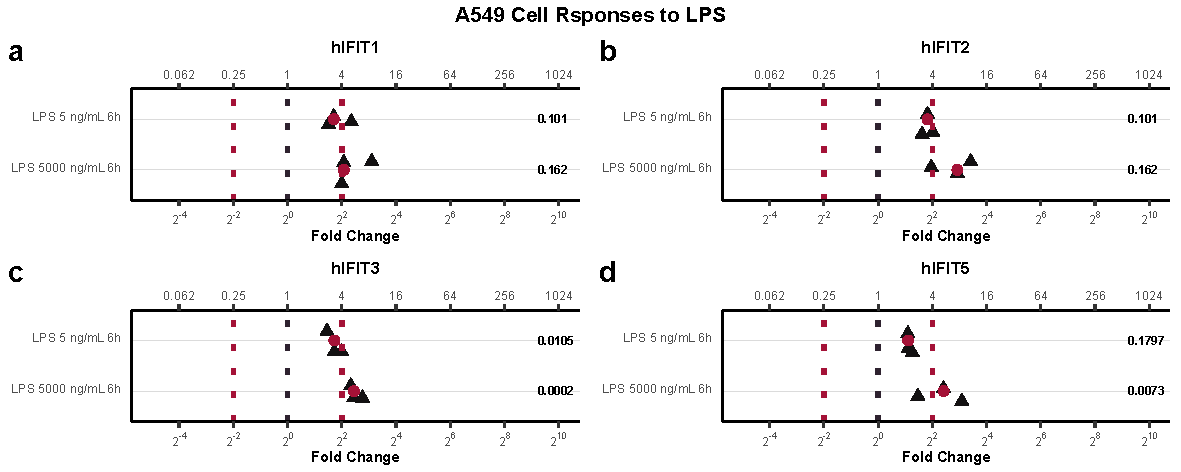
\includegraphics[width=1\linewidth]{06. Chapter 1/Figs/01. Induction/03. a549_treat_lps.pdf}
    \caption[qPCR Analysis of A549 \textit{hIFIT} Response to LPS.]{\textbf{qPCR Analysis of A549 \textit{hIFIT} Response to LPS.} The relative abundance of (a) \textit{hIFIT1}, (b) \textit{hIFIT2}, (c) \textit{hIFIT3}, and (d) \textit{hIFIT5} genes, extracted from the A549 cell line, with response to lipopolysaccharide (LPS) at concentrations of 5 and 5000 ng/mL for a treatment duration of 6 hours. The shown values are relative to standardised mock values. The red circles signify median values. The black dotted line indicates mock expression, while the red dotted lines indicate biologically significant levels of induction. Numeric values signify the p-values compared to mock.}
    \label{A549 Response to LPS}
\end{figure}

In order to assess the involvement of TLR4, a receptor also responsible for detecting RSV particles, A549 cells were incubated for 6 hours with low (5 ng/mL) and high (5,000 ng/mL) concentrations of bacterial LPS, its known activator. We can see that all \textit{IFITs} respond in a concentration dependant manner but the response is the lowest out of the different stimulants used. Low-concentration LPS incubation causes biologically insignificant induction of all \textit{hIFITs} of 2-fold for \textit{hIFIT5} and 3-fold for the other \textit{IFITs}. The high concentration on the other hand yields biologically significant induction levels of 4-8 fold induction. All \textit{hIFIT} values had normal distributions and unequal variance other than \textit{hIFIT3}, which had normal distribution and normal variance.

\begin{figure}
    \centering
    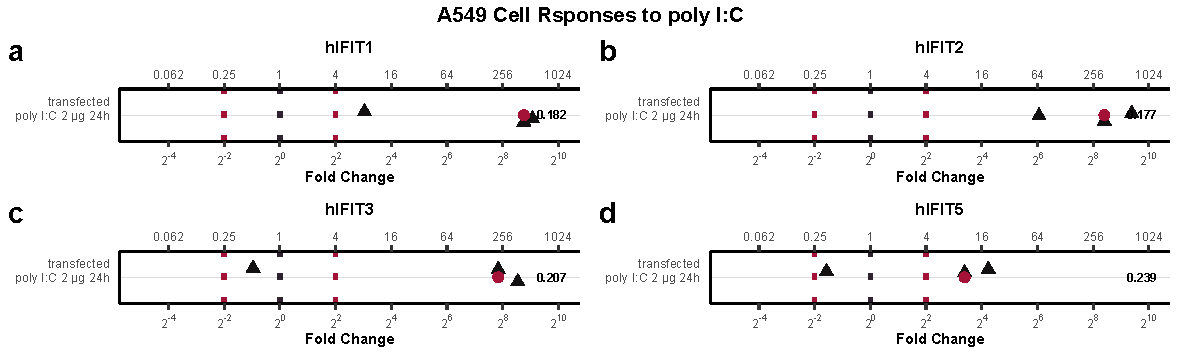
\includegraphics[width=1\linewidth]{06. Chapter 1/Figs/01. Induction/04. a549_treat_polyic.pdf}
    \caption[qPCR Analysis of A549 \textit{hIFIT} Response to Transfected poly I:C.]{\textbf{qPCR Analysis of A549 \textit{hIFIT} Response to Transfected poly I:C.} The relative abundance of (a) \textit{hIFIT1}, (b) \textit{hIFIT2}, (c) \textit{hIFIT3}, and (d) \textit{hIFIT5} genes, extracted from the A549 cell line. The cells were transfected with 2 \(\mu\)g of poly I:C for 24 hours. The shown values are relative to standardised mock values. The red circles signify median values. The black dotted line indicates mock expression, while the red dotted lines indicate biologically significant levels of induction. Numeric values signify the p-values compared to mock.}
    \label{A549 Response to poly I:C}
\end{figure}

When A549 cells were transfected with 2\(\mu\)g of poly I:C for 24 hours we were able to observe the biggest induction compared to the other inducers previously used (Figure \ref{A549 Response to poly I:C}). As with the other inducers, hIFIT1 induction is the greatest (circa 500-fold), followed by \textit{hIFIT2} and \textit{hIFIT3} with 300-fold and 200-fold responses respectively, with \textit{hIFIT5} trailing behind with the lowest response of only 10-fold. This again suggests that \textit{hIFIT5} seems to have differential transcriptomic regulation compared to the other genes of the \textit{IFIT} family. All \textit{hIFIT} values had normal distributions and unequal variance.

\begin{figure}
    \centering
    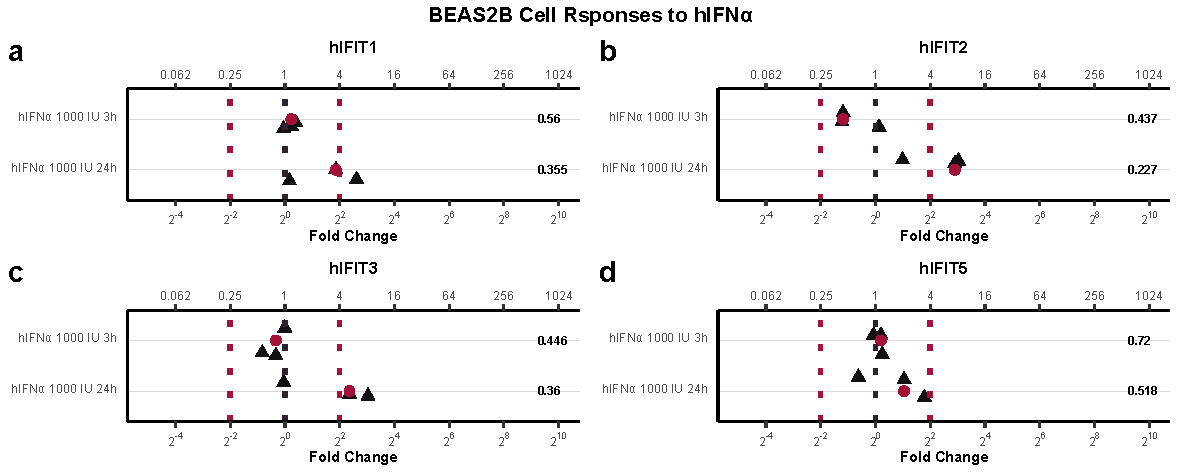
\includegraphics[width=1\linewidth]{06. Chapter 1/Figs/01. Induction/09. beas2b_ifna.pdf}
    \caption[qPCR Analysis of BEAS-2B \textit{hIFIT} Response to hIFN\(\alpha\).]{\textbf{qPCR Analysis of BEAS-2B \textit{hIFIT} Response to hIFN\(\alpha\).} The relative abundance of (a) \textit{hIFIT1}, (b) \textit{hIFIT2}, (c) \textit{hIFIT3}, and (d) \textit{hIFIT5} genes, extracted from the BEAS-2B cell line, with response to human interferon alpha (IFN\(\alpha\)) at a concentration of 1000 IU per mL for a treatment duration of 3 or 24 hours. The shown values are relative to standardised mock values. The red circles signify median values. The black dotted line indicates mock expression, while the red dotted lines indicate biologically significant levels of induction. Numeric values signify the p-values compared to mock.}
    \label{BEAS-2B responses to hIFNa}
\end{figure}

Lastly, we validated the human interferon alpha induction data in a more biologically relevant cell line, BEAS-2B. Established from bronchial epithelial biopsies from healthy samples, and later immortalised using the transfection of cyclin-dependent kinase 4 and human telomerase reverse transcriptase, these cells are an invaluable tool in the field of bronchial development and pathogenesis (\cite{Ramirez2004ImmortalizationOncoproteins}). After the treatment with human interferon alpha at concentrations of 1,000 IU/mL for 3 hours, we can see that this stimulation was not sufficient to induce the expression of any human \textit{IFIT} (Figure \ref{BEAS-2B responses to hIFNa.}). However, when the cells were stimulated for 24 hours we can observe induction above biological significance for \textit{hIFIT1}, \textit{hIFIT2}, and \textit{hIFIT3}, with 4-fold, 8-fold, and 5-fold increase respectively. \textit{hIFIT5} shows only 2-fold median induction, which could be caused by the intrinsic variability of the assay. So as we observed with the A549 cell line, \textit{hIFIT5} behaves in discord with the other human \textit{IFITs}. All \textit{hIFIT} values had normal distributions and unequal variance.


\subsubsection{Human \textit{IFITs} Responses to Human RSV} \label{Human \textit{IFITs} Responses to Human RSV}
After successfully confirming the \textit{IFIT} induction competency of  our workhorse cell line A549 as well as in the more physiologically relevant cell line BEAS-2B, we turn our attention to assessing the effect of human RSV infection on \textit{hIFIT} induction. To date, no studies have ever investigated this. Initially, we wanted to assess the effect of low, medium and high (0.1, 1, and 2 MOI respectively) infections as well as short and long-term infections (24 and 48 HPI respectively) on \textit{hIFIT} induction. My colleagues in the Viral Glycoproteins from the Pirbright Institute routinely perform hRSV infections of both A549 and BEAS-2B cell lines and thus the knowledge of what constitutes low and high MOI infection, as well as what short and long infection periods are widely known and available (I GUESS SOME CITATION HERE).  The virus was prepared and quantified as described in Section \ref{Virus Propagation and Production} and Section \ref{Virus Quantification by TCID50 Assay}. Briefly, infected cells were sonicated, cell debris was separated by centrifugation and virus-containing supernatant was gathered and titred. A549 cells were infected with the hRSV-containing supernatant at multiplicities of infection (MOI) of 0.1, 1,  and 2. Total mRNA was collected from the samples either 24 or 48 hours post-infection (HPI) and converted to complementary DNA, as described in Section \ref{RNA Extraction and cDNA Synthesis}. This was subsequently quantified by qPCR as described in Section \ref{Quantitative PCR} and the data analysed as described in Section \ref{Data Processing}. The responses of \textit{hIFITs} as a function of HPI and MOI can be seen in Figure \ref{A549 response to hRSV timepoints}, along with a plot quantifying human \textit{RSV N} mRNA as a control for viral replication. The relative quantification values of \textit{RSV N} has to be taken with a grain of salt as it is being compared to mock-infected samples that should have no \textit{RSV N} mRSN present. As a result, the actual relative values are dependent on the Ct values detected in the mock. 
 

\begin{figure}
    \centering
    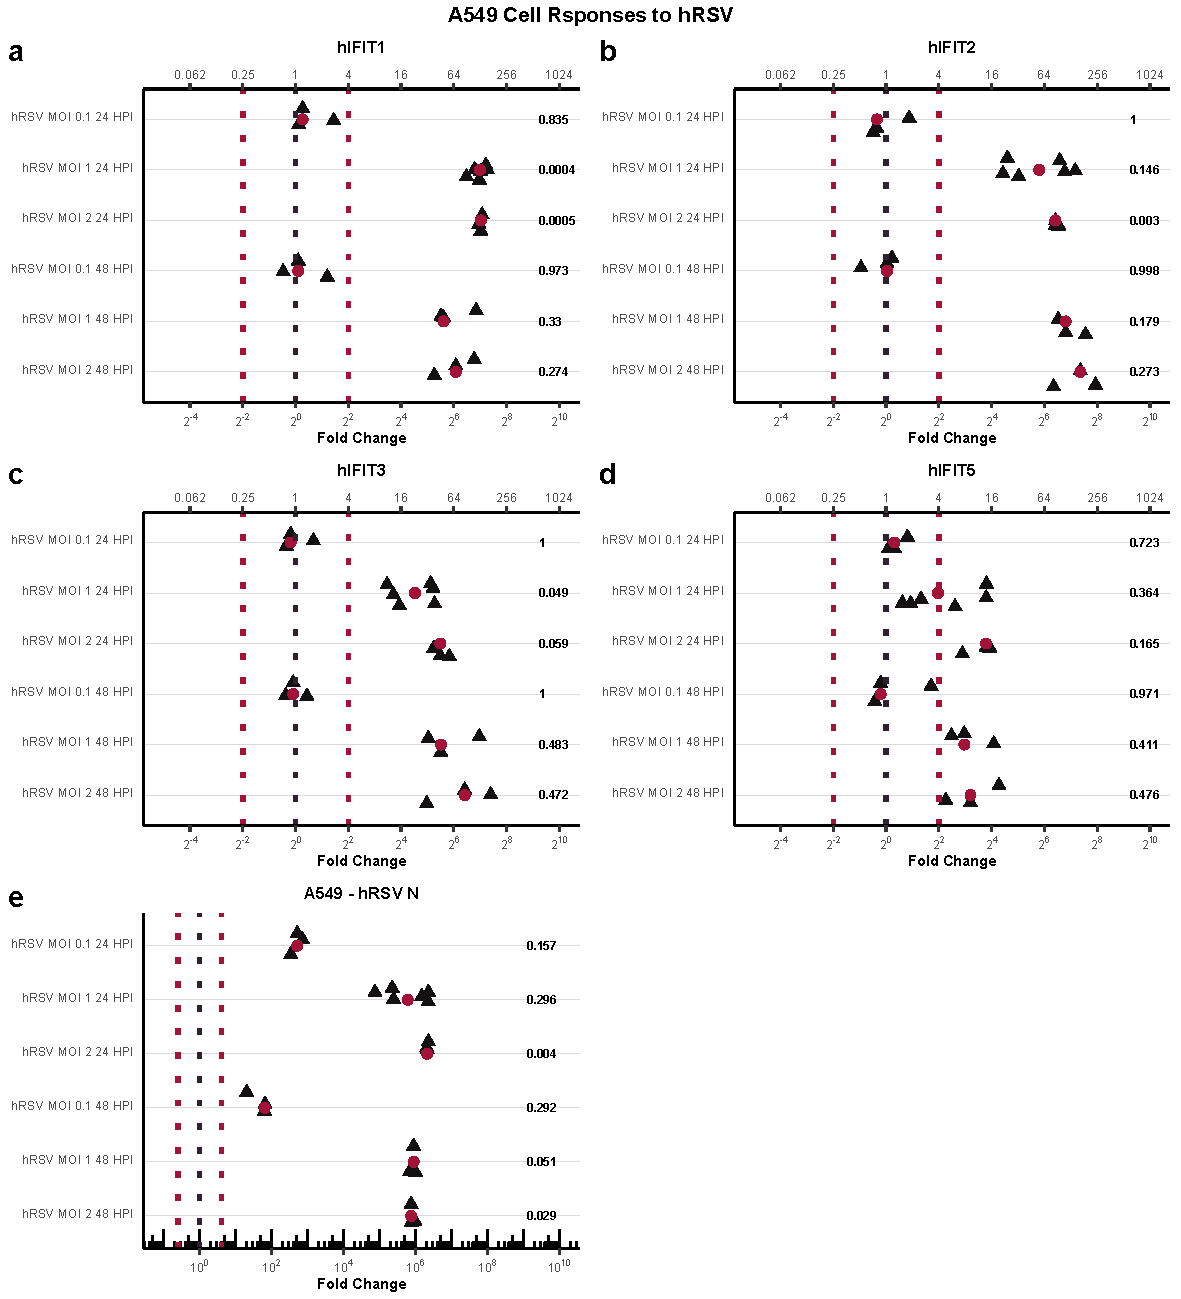
\includegraphics[width=1\linewidth]{06. Chapter 1/Figs/01. Induction/05. a549_hrsv_timepoints.pdf}
    \caption[A549 \textit{hIFIT} Response to hRSV as a Function of Time and MOI.]{\textbf{A549 \textit{hIFIT} Response to hRSV as a Function of Time and MOI.} The relative abundance of (a) \textit{hIFIT1}, (b) \textit{hIFIT2}, (c) \textit{hIFIT3}, (d) \textit{hIFIT5}, and (e) \textit{hRSV N} genes, extracted from A549 cell line following infection with human RSV at MOI of either 0.1, 1, or 2 for either 24 or 48 hours post-infection. The shown values are relative to standardised mock values. The red circles signify median values. The black dotted line indicates mock expression, while the red dotted lines indicate biologically significant levels of induction. Numeric values signify the p-values compared to mock.}
    \label{A549 response to hRSV timepoints}
\end{figure}


First of all, we can observe low MOI infection, although causing a productive infection as seen by \textit{hRSV N} mRNA relative quantification, did not yield any relative change of \textit{hIFIT} levels, suggesting that their induction is dependant not solely on the viral replication, but on the underlying magnitude of infection. In general, MOI 2 infection yields higher induction for all \textit{hIFITs}, although the magnitude is comparable with MOI 1 infections. \textit{hIFIT1} is induced the highest out of the other genes at 24 HPI, with both MOI 1 and 2 reaching 120-fold induction levels, while the induction magnitude diminishes slightly at 48 HPI, where infections at MOI 1 and 2 yield 50-fold and 80-fold median induction values. As seen previously in Section \ref{Human IFIT Responses to Known Activators of Innate Immune Response}, \textit{hIFIT2} and \textit{hIFIT3} display very similar trends of induction (with the only difference being \textit{hIFIT2} responses being 2 times the ones of \textit{hIFIT3}) for all the conditions tested here. In more detail, 24 HPI \textit{hIFIT2} gets induced 60-fold and 90-fold to the MOI of 1 and 2 respectively, while at 48 HPI the median induction magnitude increases to 100-fold and 120-fold respectively. This makes \textit{hIFIT2} the highest induced \textit{hIFIT} at 48 HPI. This also suggest that the induction dynamics of \textit{hIFIT1} differ from those of \textit{hIFIT2} and \textit{hIFIT3}. With regards to \textit{hIFIT5}, it displays the lowest, albeit still biologically significant induction for MOIs 1 and 2 for both time-points tested at median induction levels of 4 and 12 for 24 HPI MOIs 1 and 2 respectively, and 9 and 10 for 48 HPI MOIs 1 and 2 respectively. 


\begin{figure}
    \centering
    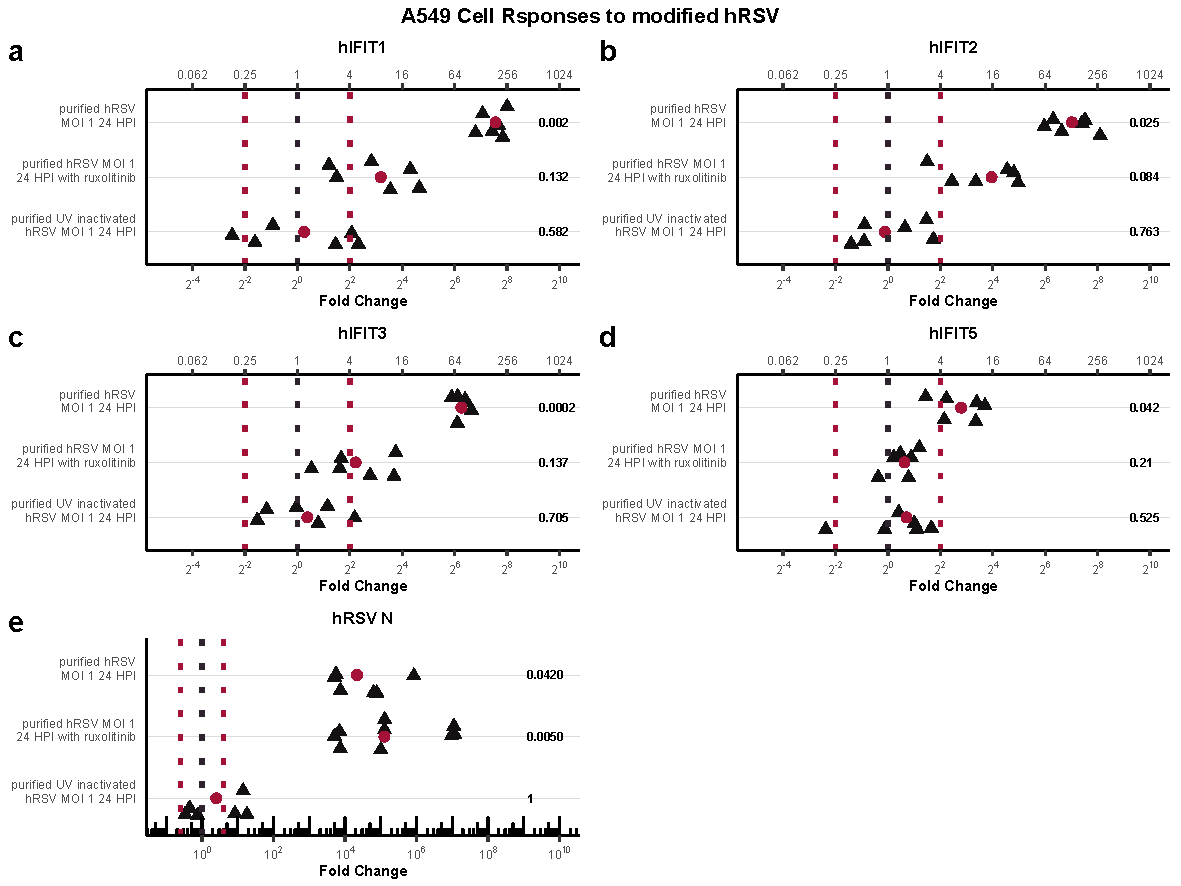
\includegraphics[width=1\linewidth]{06. Chapter 1/Figs/01. Induction/06. a549_hrsv_uv_roxo.pdf}
    \caption[The Effect of Ultra-Purification, UV-Inactivation and INFR Inhibition on \textit{hIFIT} Induction Following hRSV Infection in A549.]{\textbf{The Effect of Ultra-Purification, UV-Inactivation and INFR Inhibition on \textit{hIFIT} Induction Following hRSV Infection in A549.} The relative abundance of (a) \textit{hIFIT1}, (b) \textit{hIFIT2}, (c) \textit{hIFIT3}, (d) \textit{hIFIT5}, and (e) \textit{hRSV N} genes, extracted from A549 cell line following infection with ultra-purified hRSV at MOI 1 for 24 hours. The cells were either treated with the virus alone (first row), or with the virus and 5 nM of ruxolitinib (interferon receptor inhibitor) during the whole infection period (second row), or with UV-inactivated hRSV (last row). The shown values are relative to standardised mock values. The red circles signify median values. The black dotted line indicates mock expression, while the red dotted lines indicate biologically significant levels of induction. Numeric values signify the p-values compared to mock.}
    \label{The effect of ultra-purification, UV-inactivation and INFR inhibition on hIFIT induction following hRSV infection in A549}
\end{figure}
After confirming and concluding that human RSV infection indeed induces \textit{hIFIT} mRNA expression, we wanted to investigate the underlying induction principles. We wanted to investigate if the induction observed is indeed caused by human RSV detection and not by any other contaminants present in the virus prep such as cytokines, chemokines, and other stimulants. To do this, we created ultra-purified hRSV preps by ultra-centrifugation on a discontinuous sucrose cushion, as described in Section \ref{Virus Propagation and Production}. We also wanted to test if it is predominately the infected cells that have the \textit{hIFIT} expression increased as a defence mechanism to acute infection, or if the infected cells stimulate the \textit{hIFIT} expression in neighbouring cells as a prophylactic against the infection, or both. To test this, after the infection procedure, we incubated the cells with 5 nM of ruxolitinib, a well established small molecule JAK/STAT inhibitor, as is described in Section \ref{Viral Infections, UV-Inactivation and Ruxolitinib Treatment}. Based on the observations from Figure \ref{A549 response to hRSV timepoints} we used MOI of 1, 24 HPI to ensure sufficient \textit{hIFIT} induction, while decreasing the stress of the cells.  Lastly, we also hypothesised that viral replication is required for \textit{hIFIT} expression. To test this, some ultra-purified hRSV samples were UV-inactivated by a UV-cross-linker, as described in Section \ref{Viral Infections, UV-Inactivation and Ruxolitinib Treatment}.

The results of the experiment can be seen in Figure \ref{The effect of ultra-purification, UV-inactivation and INFR inhibition on hIFIT induction following hRSV infection in A549}. We can see that although purified hRSV infection yielded lower induction compared to what was observed in Figure \ref{A549 response to hRSV timepoints} with regards to hRSV MOI 1 24 HPI infection (\(10^6\)-fold to \(10^{4.5}\)-fold), it induced all \textit{hIFITs}, even to higher mounts that what was seen with crude-extracted virus. In more detail, \textit{hIFIT1} was induced the highest at 180-fold (compared to 120-fold observed previously), closely followed by \textit{hIFIT2}, which median induction was at 180-fold (compared to 80-fold observed previously). \textit{hIFIT3} induction was 75-fold, double what was seen previously with crude extracted hRSV, while \textit{hIFIT5} median induction was 6-fold, a very comparable level to 4-fold that was observed previously. Regardless of the absolute magnitude of the relative values, this data suggest that the main driving force in hRSV presence and not contaminants in the viral prep. With regards to the effect of JAK/STAT inhibitor ruxolitinib, its presence diminished induction of all \textit{hIFITs}. \textit{hIFIT1}, \textit{hIFIT2}, and \textit{hIFIT3} maintained median induction values above the biologically significant threshold at 8, 10, and 5-fold respectively, while \textit{hIFIT5} showed only minimal median induction value of only 1.5-fold. We can also observe an order of magnitude more \textit{hRSV N} mRNA detection, suggesting that inhibiting interferon signalling is beneficial for the virus, which makes sense. Lastly, we assessed how a detection of non-replicative hRSV particles contribute to \textit{hIFIT} induction. UV-cross-linking of hRSV inhibited viral replication, as can be seen by the {hRSV N} mRNA quantification. This in fact prevented induction of all the \textit{hIFITs}, suggesting that TLR4 sensing of RSV particle is not sufficient to initiate signalling cascades that would lead to \textit{hIFIT} induction. All together, this data suggest that hRSV particles indeed drive the \textit{hIFIT} induction, however, they have to be replication competent. Additional essential aspect is the presence of functional interferon signalling cascades and the underlying paracrine interferon signalling initiated by infected cells in order to protect its neighbours.

\begin{figure}
    \centering
    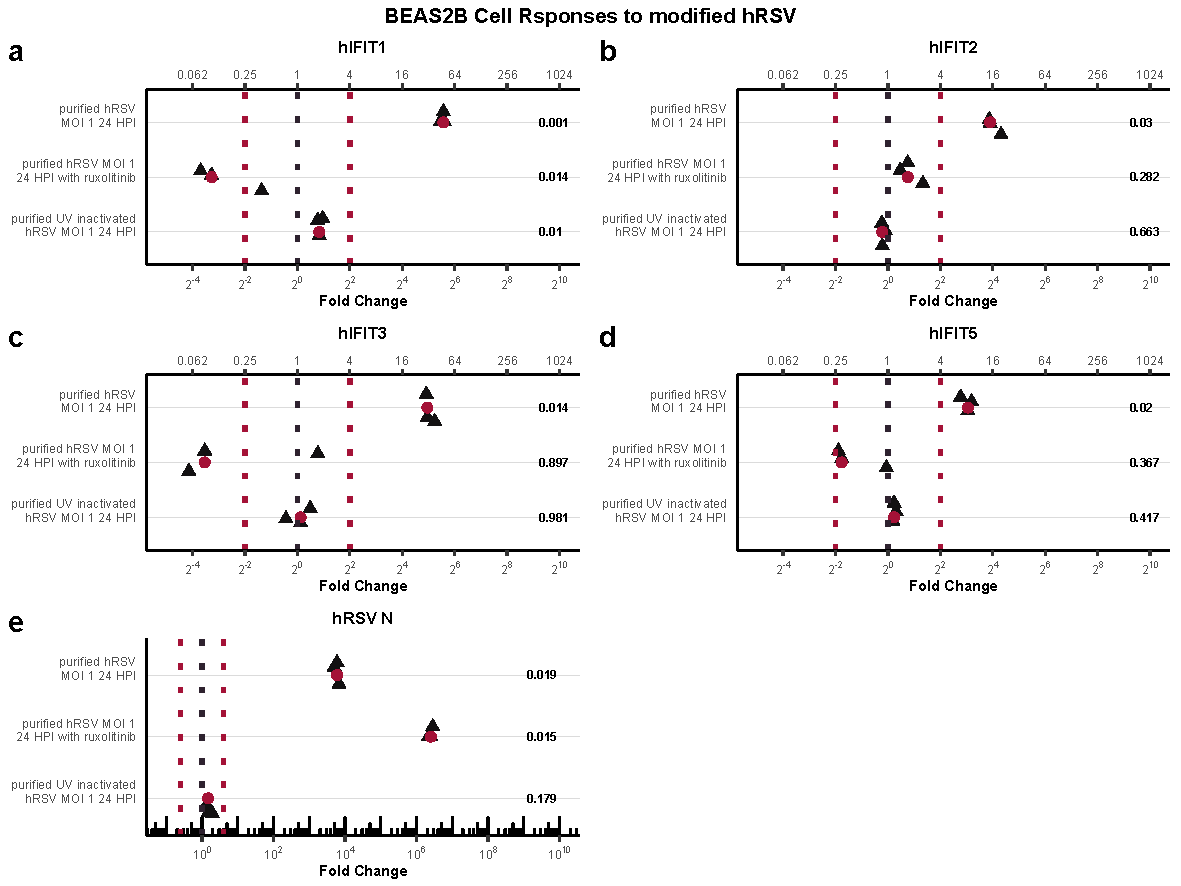
\includegraphics[width=1\linewidth]{06. Chapter 1/Figs/01. Induction/10. beas2b_hrsv.pdf}
    \caption[The Effect of Ultra-Purification, UV-Inactivation and INFR Inhibition on \textit{hIFIT} Induction Following hRSV Infection in BEAS-2B.]{\textbf{The Effect of Ultra-Purification, UV-Inactivation and INFR Inhibition on \textit{hIFIT} Induction Following hRSV Infection in BEAS-2B.} The relative abundance of (a) \textit{hIFIT1}, (b) \textit{hIFIT2}, (c) \textit{hIFIT3}, (d) \textit{hIFIT5} and (e) \textit{hRSV N} genes, extracted from BEAS-2B cell line following infection with ultra-purified hRSV at MOI 1 for 24 hours. The cells were either treated with the virus alone (first row), or with the virus and 5 nM of ruxolitinib (interferon receptor inhibitor) during the whole infection period (second row), or with UV-inactivated hRSV (last row). The shown values are relative to standardised mock values. The red circles signify median values. The black dotted line indicates mock expression, while the red dotted lines indicate biologically significant levels of induction. Numeric values signify the p-values compared to mock.}
    \label{The effect of ultra-purification, UV-inactivation and INFR inhibition on hIFIT induction following hRSV infection in BEAS-2B}
\end{figure}

Next we validated the findings using BEAS-2B cell line. We recreated the experiment from Figure \ref{The effect of ultra-purification, UV-inactivation and INFR inhibition on hIFIT induction following hRSV infection in A549} and the results can be seen in Figure \ref{The effect of ultra-purification, UV-inactivation and INFR inhibition on hIFIT induction following hRSV infection in BEAS-2B}. All \textit{hIFITs} are induced to biologically significant levels by the infection of ultra-purified hRSV infection by 40, 15, 32, and 7-fold for \textit{hIFIT1}, \textit{hIFIT2}, \textit{hIFIT3}, and \textit{hIFIT5} respectively. These responses are also significantly higher than what was observed with human interferon alpha treatment (Figure \ref{BEAS-2B responses to hIFNa}). In line to what we have seen in A549 cell line, \textit{hIFIT1} is the highest induced, while \textit{hIFIT5} responds the worst to the infection. Interestingly, \textit{hIFIT3} median induction is higher than the one of \textit{hIFIT2}. When looking at the effect of ruxolitinib we can see that it prevented the induction of \textit{hIFIT2} and actually significantly decreased the relative levels of \textit{hIFIT1}, \textit{hIFIT3}, and \textit{hIFIT5} to the levels of \(2^{-3}\), \(2^{-3.5}\), and \(2^{-2}\) respectively. This suggest that not only is the interferon signalling required for \textit{hIFIT2} induction, it is vital for the maintenance  of basal \textit{hIFIT1}, \textit{hIFIT3}, and \textit{hIFIT5} levels in this cell line. 

uv data identical to a549

The trends seen with A549 are kind of recapitulated.




\myparagraph{Validation by Comparing to the Proteomic Dataset} \label{Validation by Comparing to the Proteomic Dataset}
Who, what and why it was done
Cite the bioArchive paper (\cite{Jobe2023ViralCondensates})

Proteomics dataset from Dalan’s lab looking at differential enrichment of proteins between membrane and cytosolic fractures. It confirms that in A549 (I think) IFITs 1 (series 1), 2 (series 2) and 3 (series 3) are induced in the cytosolic fraction at protein level 



I have attached the IFIT data that came out of the screen. There were no hits for IFIT5. C=cytoplasmic fractions M= Membrane fraction, 24=24 hours post infection, 48=48 hours post infection
In the screen I had to discard data for IFIT1,3 and 5. The data for IFIT2 was good though, IFIT2 had a Z-score of -1. So it only just made the cut off for being inhibitory by the criteria of the screen. Still could be worth a try though.



\begin{figure}
    \centering
    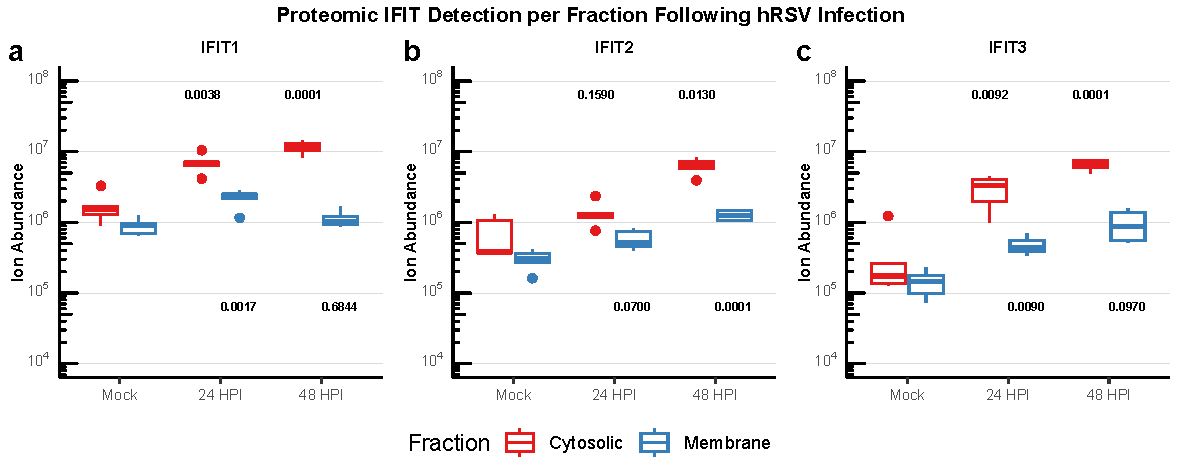
\includegraphics[width=1\linewidth]{06. Chapter 1/Figs/01. Induction/13. merged_proteomics.pdf}
    \caption[Human IFIT proteins detected per fraction.]{\textbf{Human IFIT proteins detected per fraction.} The ion abundance of (a) hIFIT1, (b) hIFIT2, and (c) hIFIT3 detected per either cytosolic or membrane fraction of A549 cells which were either mock-infected, or infected with hRSV MOI # for either 24 or 48 hours.There were no hits for IFIT5. This data is from a proteomic study, published in \cite{Jobe2023ViralCondensates}. Samples are composed of biological quintuplicates. Numeric values signify the p-values compared to mock the respective mock, i.e. top numbers for cytosolic fraction, bottom for membrane fraction.}
    \label{Human IFIT proteomics.}
\end{figure}


\subsubsection{Human \textit{IFITs} Responses to bRSV} \label{Human IFITs Responses to bRSV}
How were viruses harvested and cells infected \newline
Justify moi and timepoints

\begin{figure}
    \centering
    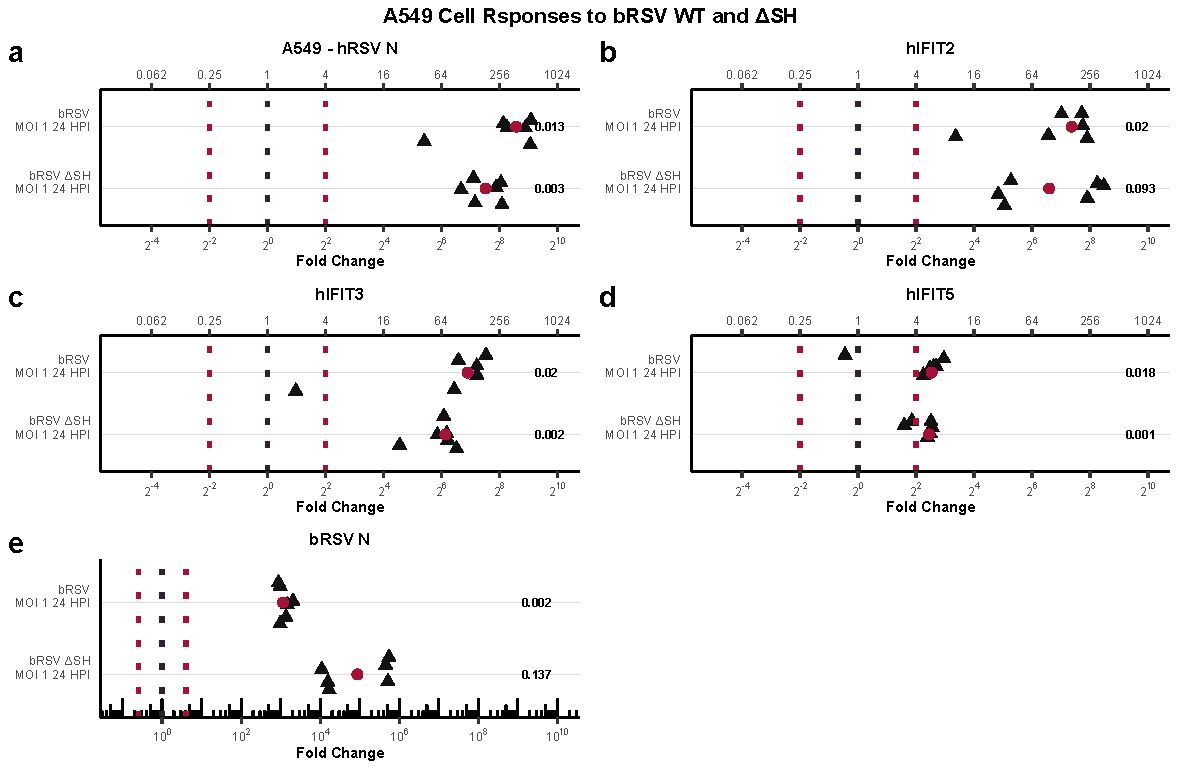
\includegraphics[width=1\linewidth]{06. Chapter 1/Figs/01. Induction/07. a549_brsv_moi1.pdf}
    \caption[A549 \textit{hIFIT} Response to WT and \(\Delta\)SH bRSV Infection.]{\textbf{A549 \textit{hIFIT} Response to WT and \(\Delta\)SH bRSV Infection.} The relative abundance of (a) \textit{hIFIT1}, (b) \textit{hIFIT2}, (c) \textit{hIFIT3}, (d) \textit{hIFIT5} and (e) \textit{bRSV N} genes, extracted from A549 cell line following infection with WT or \(\Delta\)SH bRSV at MOI 1, 24 HPI.  The shown values are relative to standardised mock values. The red circles signify median values. The black dotted line indicates mock expression, while the red dotted lines indicate biologically significant levels of induction. Numeric values signify the p-values compared to mock.}
    \label{Responses of A549 to bRSV WT and dSH.}
\end{figure}



Infection cells with WT bRSV induces IFITs more than infection with hRSV.  Infection with mutant bRSV viruses (at normal and low MOI) induces human IFITs but IFIT5, which is only responsive to MOI 1 dSH bRSV and MOI 0.001 dNS1/2 bRSV.

The low MOI infection causing induction are interesting as low MOI hRSV did not cause induction. Maybe bRSV is more potent of A549 cells?

\begin{figure}
    \centering
    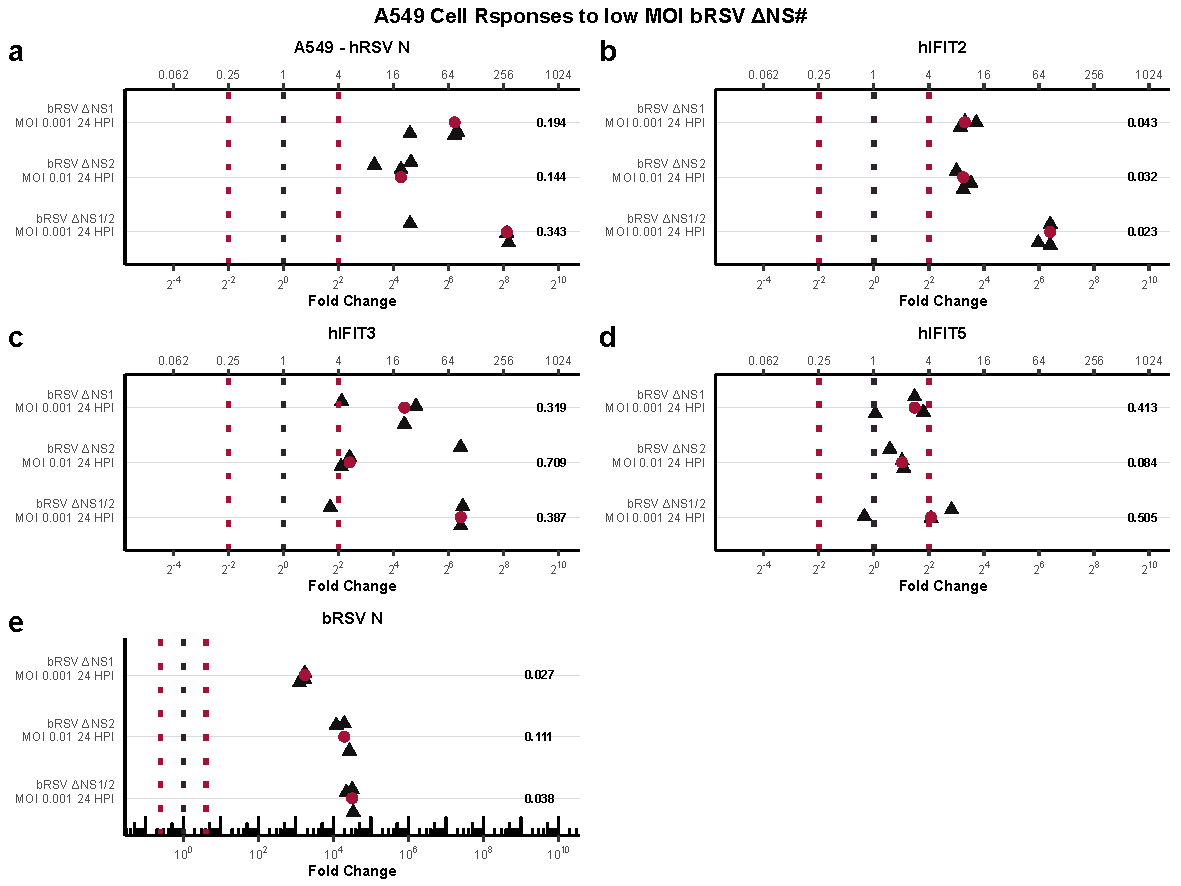
\includegraphics[width=1\linewidth]{06. Chapter 1/Figs/01. Induction/08. a549_brsv_dns.pdf}
    \caption[A549 \textit{hIFIT} Response to Low MOI \(\Delta\)NSs bRSV Infection.]{\textbf{A549 \textit{hIFIT} Response to Low MOI \(\Delta\)NSs bRSV Infection.} The relative abundance of (a) \textit{hIFIT1}, (b) \textit{hIFIT2}, (c) \textit{hIFIT3}, (d) \textit{hIFIT5} and (e) \textit{bRSV N} genes, extracted 24 HPI from A549 cell line following infection with bRSV \(\Delta\)NS1, \(\Delta\)NS2, and \(\Delta\)NS1/2 at MOIs of 0.001, 0.01, and 0.001 respectively. The shown values are relative to standardised mock values. The red circles signify median values. The black dotted line indicates mock expression, while the red dotted lines indicate biologically significant levels of induction. Numeric values signify the p-values compared to mock.}
    \label{Responses of A549 to bRSV dNSs.}
\end{figure}

some text some text some text

\begin{figure}
    \centering
    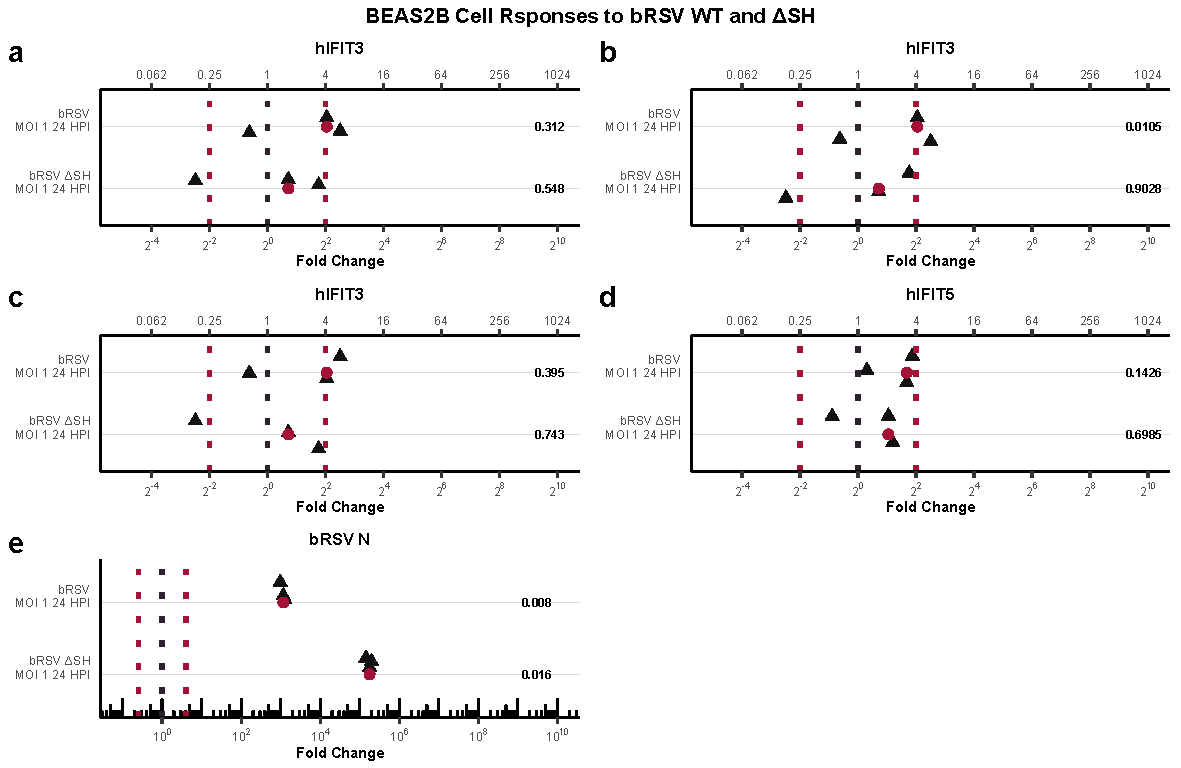
\includegraphics[width=1\linewidth]{06. Chapter 1/Figs/01. Induction/11. beas2b_brsv_moi1.pdf}
    \caption[BEAS-2B \textit{hIFIT} Response to WT and \(\Delta\)SH bRSV Infection.]{\textbf{BEAS-2B \textit{hIFIT} Response to WT and \(\Delta\)SH bRSV Infection.} The relative abundance of (a) \textit{hIFIT1}, (b) \textit{hIFIT2}, (c) \textit{hIFIT3}, (d) \textit{hIFIT5} and (e) \textit{bRSV N} genes, extracted from BEAS-2B cell line following infection with WT or \(\Delta\)SH bRSV at MOI 1, 24 HPI.  The shown values are relative to standardised mock values. The red circles signify median values. The black dotted line indicates mock expression, while the red dotted lines indicate biologically significant levels of induction. Numeric values signify the p-values compared to mock.}
    \label{BEAS-2B responses to bRSV WT and dSH.}
\end{figure}

some text some text some text some text

\begin{figure}
    \centering
    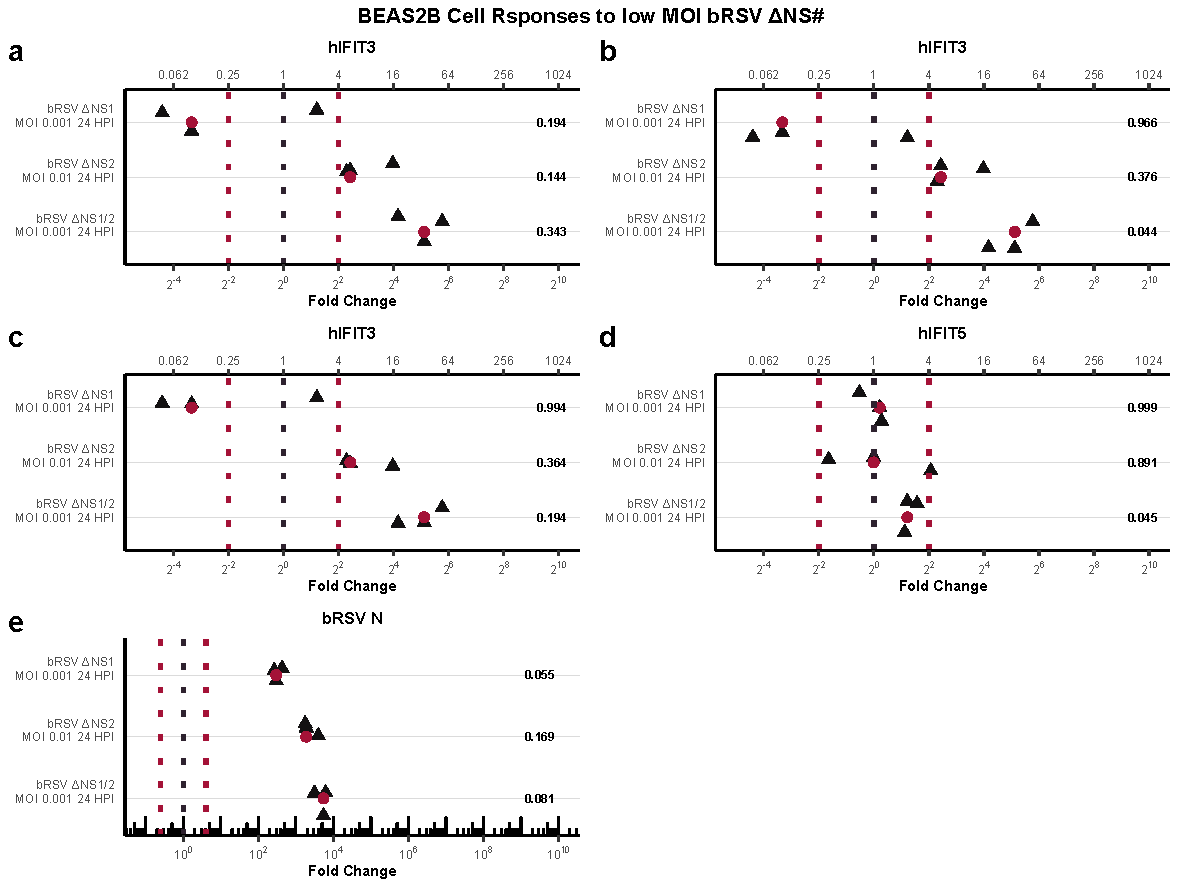
\includegraphics[width=1\linewidth]{06. Chapter 1/Figs/01. Induction/12. beas2b_brsv_dns.pdf}
    \caption[BEAS-2B \textit{hIFIT} Response to Low MOI \(\Delta\)NSs bRSV Infection.]{\textbf{BEAS-2B \textit{hIFIT} Response to Low MOI \(\Delta\)NSs bRSV Infection.} The relative abundance of (a) \textit{hIFIT1}, (b) \textit{hIFIT2}, (c) \textit{hIFIT3}, (d) \textit{hIFIT5} and (e) \textit{bRSV N} genes, extracted 24 HPI from BEAS-2B cell line following infection with bRSV \(\Delta\)NS1, \(\Delta\)NS2, and \(\Delta\)NS1/2 at MOIs of 0.001, 0.01, and 0.001 respectively. The shown values are relative to standardised mock values. The red circles signify median values. The black dotted line indicates mock expression, while the red dotted lines indicate biologically significant levels of induction. Numeric values signify the p-values compared to mock.}
    \label{BEAS-2B responses to bRSV dNSs.}
\end{figure}


some last text and thats it for this Chapter

IFIT5 does not get induced by any bRSV infection tried (probably because IFIT5 has either basally higher levels and thus the same end mRNA concentration equates to lower induction or because it is really not induced by bRSV (although the IFITs should have the same promoters)). Low MOI infection (0.001 and 0.01) of dNS1 and dNS2 bRSV induces IFITs 1,2 and 3, while dSH MOI1 and dNS1/2 MOI 0.001 does not. 

\subsubsection*{Summary} \label{Summary-human-induction}
Interestingly, the maximal induction of \textit{hIFIT5} observed in this study seems to be 10-16 fold, a order of magnitude lower of what is observed for the other \textit{hIFIT}.